\documentclass[a1paper,portrait,fontscale=0.45]{baposter}

\usepackage{relsize}		% For \smaller
\usepackage{url}			% For \url
\usepackage[font=small,labelfont=bf]{caption}
\usepackage{multicol}

\definecolor{bordercol}{RGB}{0, 92, 132}
\definecolor{headercol1}{RGB}{81, 98, 111}
\definecolor{headercol2}{RGB}{81, 98, 111}
\definecolor{headerfontcol}{RGB}{0,0,0}
\definecolor{boxcolor}{RGB}{255, 255, 255}
\definecolor{backcol}{RGB}{0, 92, 132}
%\color{white}

\hyphenation{system without program examined environment modelling practices}

\newcommand{\compresslist}{
	\setlength{\itemsep}{1pt}
	\setlength{\parskip}{0pt}
	\setlength{\parsep}{0pt}
}

\begin{document}

\begin{poster}
{
	headerfont=\Large\bf\color{white},
	borderColor=bordercol,
	headerColorOne=headercol1,
	headerColorTwo=headercol2,
	headerFontColor=headerfontcol,
	headershape = rectangle,
	textborder = none,
	headerborder = none,
	boxColorOne=boxcolor,
	bgColorOne=backcol,
	background = plain,
	columns=2,
	headerheight=0.15\textheight
}
{

}
{
	\color{white}{Investigating the feasibility and worth\\of migrating legacy systems}
}
{
	\vspace{1em}
	\color{white}{Candidate: Patrick Naish - pn3g10@zepler.net\\
	Supervisor: Prof. Michael Butler - mjb@ecs.soton.ac.uk}
}
{
	
\includegraphics[keepaspectratio=true, height=5em]{uos.png}
}

\renewcommand{\familydefault}{\sfdefault}

\headerbox{Introduction}{name=introduction,column=0,row=0, span=2}{
Mainframe computing has long been the backbone of technological industry. Despite having fallen out of favour in deference to the modern client-server style of interaction, mainframe software still underpins a vast amount of modern systems. Despite the fact that there were an estimated 200 billion lines of COBOL in use in 2008 \cite{Datamonitor2008}, COBOL is widely considered to be a dead language, and the fact that young computer scientists are primarily taught languages such as Java \cite{Sneed2013} and Python means that many are unwilling to learn older languages. Those developers who do know the languages required to maintain legacy mainframe systems are rapidly reaching the age of retirement and leaving the industry. Thus, it is important to find a means by which to modernise legacy systems to preserve their functionality, while allowing for practical future maintenance.
}

\headerbox{Approaches to modernisation}{name=approaches,column=0,below=introduction, span=1}{
The four main approaches suggested by Almonaies et al. \cite{Almonaies2010} are:
\begin{description}
	\compresslist
	\item[Replacement] The original system is rewritten in a new language or replaced with an off-the-shelf solution.
	\item[Reengineering] Modern functionality is reverse-engineered into the legacy system.
	\item[Wrapping] An interface is created to access legacy components as services without changing them.
	\item[Migration] The legacy system is transitioned into a modern environment while retaining functionality.
\end{description}

The most common end-goal for modernisation is to be able to access the system as a \textbf{Web Service}\footnote{\footnotesize See \url{http://www.w3.org/TR/wsdl}}.
}

\headerbox{Tools}{name=tools,column=0,below=approaches}{
There are various tools available for aiding the modernisation effort. The examined tools fell into two categories: those for \textbf{analysis} of systems, and those for the actual \textbf{migration}.
\vspace{1em}

An example of a tool for analysis is \textbf{COBAudit}, which collects metrics about COBOL programs \cite{Sneed2009}. These metrics can then be used to assess the complexity of a program, and said program's suitability for modernisation. \textbf{ARMIN} is a somewhat more specialised tool, which reconstructs a program's architecture from a static analysis of the code \cite{O'Brien2005}. This can be used to identify dependencies within programs, which can then inform the creation of a migration strategy.
\vspace{1em}

One set of tools for migration is \textbf{COB2WEB}, which comprises COBAudit along with COBStrip, COBWrap and COBLink \cite{Sneed2008}. \textbf{COBStrip} separates out a program into `slices', which each represent a path through the program performing a distinct function. These are used to create cut-down versions of the original program performing only those functions, allowing for each piece of functionality to be represented by a separate Web Service. To this end, \textbf{COBWrap} adds an I/O layer to sit between the legacy code and the web, and \textbf{COBLink} generates Web Service Description Language (WSDL) interfaces for the same.

\begin{center}
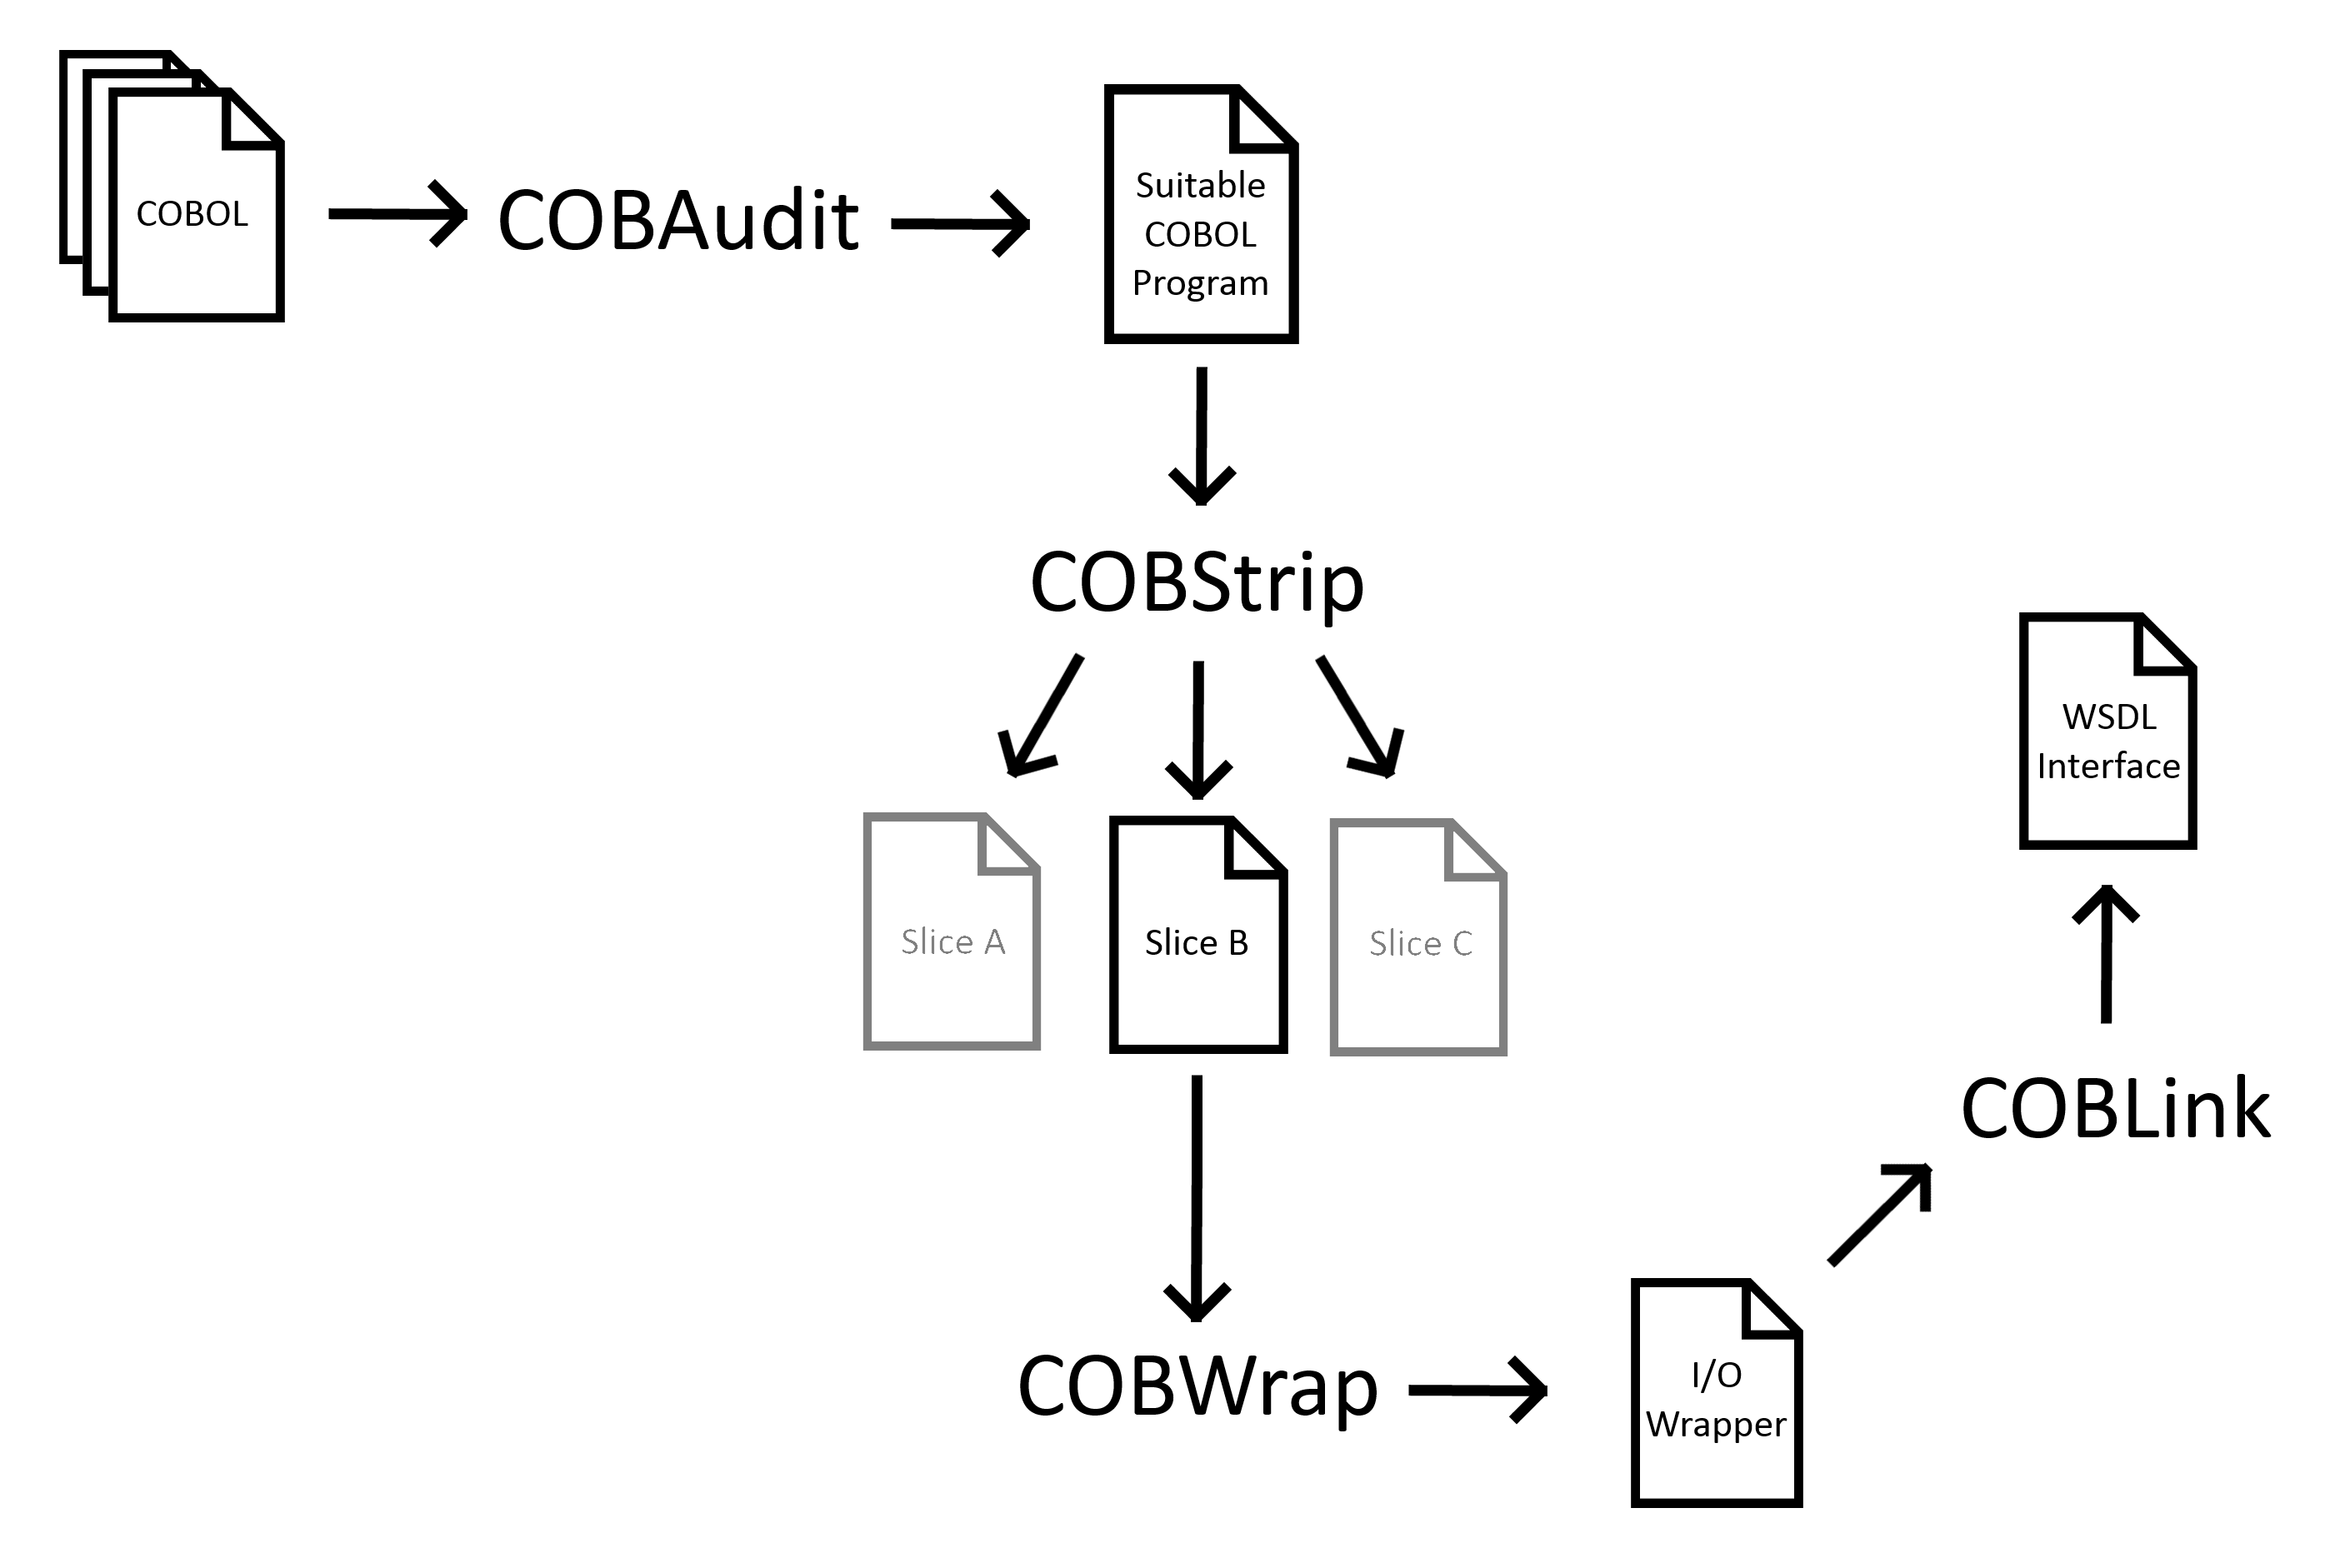
\includegraphics[keepaspectratio=true, width=19em]{cob2web.png}
\captionof{figure}{An illustration of the COB2WEB process}
\end{center}
}

\headerbox{Techniques}{name=techniques,column=1,below=introduction}{
Several techniques have been developed and tested for applying tools and practices to real-world systems. Most of those examined had been tested in at least a case study environment, although not all.
\vspace{1em}

Among these techniques is the Service-Oriented Migration and Reuse Technique (\textbf{SMART}), a process for evaluating the potential for legacy components to become services \cite{Lewis2005}. This considers not only the complexity of the system, but also factors such as the target environment and user base. This gives a more complete overview of the system and its role in the company environment than a single tool such as COBAudit.
\vspace{1em}

Another technique is \textbf{CelLEST}, developed as part of the CelLEST project \cite{Stroulia2000}. This differs from many other techniques in that, rather than attempting to understand a system's architecture through code analysis, a model of the behaviour of the system is constructed based on user interface interaction. Requiring more direct user interaction than other techniques, it does have the advantage of reducing the necessity for large-scale software engineering processes.
\vspace{1em}

The Ubiquitous Web Applications Design Framework (\textbf{UWA}) is a technique for reengineering \cite{Distante:2006:RLA:1134285.1134353}. It involves reverse-engineering of the legacy system to create `meta-models', which can then be used to create concrete models for the original system, which can in turn be used to engineer a web version of the original system.
\vspace{1em}

\textbf{Finite State Automata} have also been discussed as a potential tool for modelling user-system interactions \cite{Canfora2006}. This is to address the issue introduced when handling multiple connections as a Web Service -- namely, the underlying system may be in an unknown state when a request is received, leading to unexpected behaviour. With a finite state automaton keeping track of the state of the system, the currently available I/O operations can be modelled in the wrapper layer, thereby mitigating the issue.
}

\headerbox{Conclusion}{name=conclusion,column=1,below=techniques}{
The main issues presented to the task of system modernisation and migration are those of cost-effectiveness, maintainability and automation. The difficulty lies in assessing whether it is possible to effectively modernise a system, and the actual benefits of doing so. A business must be able to find the most appropriate approach for their situation, and balance the up-front costs of more expensive approaches, such as migration, against the poor maintainability of cheaper solutions such as wrapping. Finding a means to automate (to some degree) the process of striking said balance is vital to the future of the field, and is likely to be where the bulk of new research and development is focused.
\vspace{1em}

Overall, the available tools and techniques provide a significant basis for those wishing to attempt the modernisation of their systems, although as few have been tested widely in real-world scenarios some modifications may be needed to make them practical. New tools based on the currently existing ones are likely to emerge in future -- and, in turn, new processes based around the use of these tools.
}

\headerbox{References}{name=references,column=0,below=tools, span=2}{
	\renewcommand{\refname}{\vspace{-0.8em}}
	\bibliographystyle{plain}
	\begin{multicols}{3}
	\scriptsize
	\itemsep=-0.01em
	\bibliography{references}
	\end{multicols}
}

\end{poster}

\end{document}
